\chapter{绪论}
\label{chapter:intro}

\section{研究背景}
\label{section:background}

生物信息学是研究生物信息的采集、处理、存储、传播和解释等各方面的学科。
生物信息学可以帮助人类从海量的生物数据中挖掘内部的生理过程规律,从而指导进一步的生物学研究。在规模化实验大力发展和海量数据爆发的如今,如何有效的利用生物数据变得越来越中了。
生物信息学分为三个主要的发展阶段,前基因组时代主要建立了各种生物数据库和序列比较算法、基因组时代进行了大规模的基因测序以及目前所处的后基因组时代。
后基因组时代研究重心以生物数据分析为主,并且挖掘的层次逐渐深入。已经从对基因组直接的结构的研究逐渐转向对基因功能的研究,其中的主要侧重点包括基因组学、转录组学以及蛋白质组学等\cite{helms_principles_2019}。

蛋白质是生物细胞和组织的重要组成部分,是生命体的物质基础,也是遗传信息的直接表达手段,涉及生物体载体、免疫、激素等方方面面。蛋白质分子深度参与了组织的构成与修复、生理功能的调节和能量的供给。
蛋白质组学\cite{schubert_quantitative_2017}是在蛋白质表达层面研究生理生化功能为主的一门学科,目的是揭示蛋白质的基本生命活动规律,其中研究主要关注蛋白质结构、蛋白质丰度、蛋白质修饰以及蛋白质相互作用。

蛋自质在细胞活动中发挥着巨大的作用。但是在多数情况下单个蛋自质无法独立的执行生物功能,只有构成蛋白质复合物,才能有效的参与到细胞活动中\cite{gavin_functional_2002}。因此蛋白质复合物的结构、功能及形成方式的研究就显得尤为重要。图\ref{fig:swr1_complex}是具有染色质重塑功能的酵母SWR1复合物。
\begin{figure}[htbp]
  \centering
  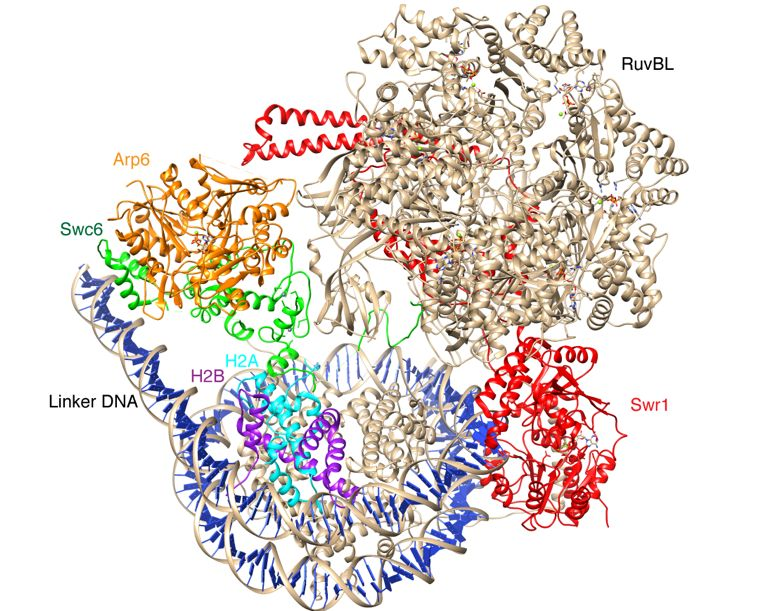
\includegraphics{SWR1_complex}
  \caption{酵母菌SWR1复合物}
  \label{fig:swr1_complex}
\end{figure}
生物实验中检测蛋白质复合物主要通过串联亲和纯化与质谱分析\cite{g_generic_1999}、酵母双杂交\cite{li_identification_1993}两种技术对蛋白质复合物进行分离和鉴定。串联亲和纯化与质谱分析通过靶蛋白标定以及自然条件下亲和纯化获取可能的蛋白质复合物,再使用质谱分析进行鉴定。酵母双杂交技术利用转录调控因子中的组件特征研究蛋白质之间的相互作用关系。虽然基于实验测定的方法具有生物学上的可解释性,但是生物实验往往条件困难、实验步骤多且成本昂贵,无法满足快速增长的研究需求。

蛋白质与生理环境存在广泛的相互作用,蛋白质复杂功能的实现同蛋白质之间、DNA与蛋白质、RNA与蛋白质的相互作用密切相关,蛋白质复合物正是一组强相关的蛋白质组合共同作用的结果。随着生物信息学的发展以及高通量技术的发展,蛋白质相互作用关系(Protein-ProteinInteraction,$PPI$,后简称为互作关系)得到了大量的补充,促成了大规模互作网络的构建\cite{butland_interaction_2005},即蛋白质相互作用网络(Protein-ProteinInteractionNetwork,$PIN$)。图\ref{fig:ppi}为酵母菌蛋白质相互作用网络。
\begin{figure}[htbp]
  \centering
  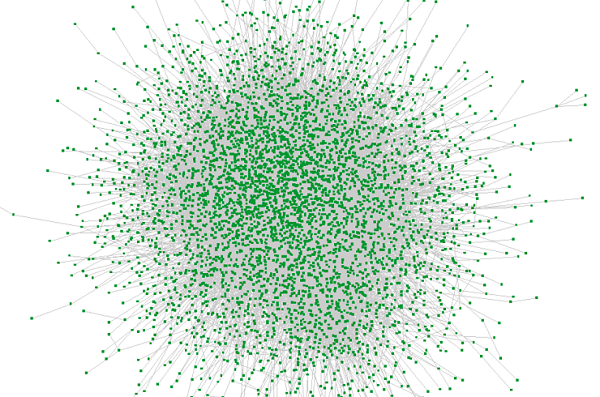
\includegraphics{ppi}
  \caption{酵母菌蛋白质相互作用网络}
  \label{fig:ppi}
\end{figure}
已知的蛋白质复合物可以视作互作网络里面的一系列子网络,因此利用图论和计算模型学习子网络的分布模式,即可在互作网络中发掘潜在的蛋白质复合物\cite{legrain_proteinprotein_2001}。利用图论的方法,蛋白质互作网络可以转换为无向图~$G=(V,E)$。其中$V$为图中结点的集合,表示所有的蛋白质,$E$为图中邻边的集合,表示所有的蛋白质互作关系。$PIN$转换为图结构之后,图论上的计算模型和深度学习方法就可以迁移到蛋白质复合物的研究中。2002年,Tong\cite{tong_combined_2002}等人提出了密集子图的假说,蛋白质复合物在$PIN$是密集链接的子图,而与其他的蛋白质连接相对稀疏。在$PIN$中预测蛋白质复合物的问题就转换为了密集子图的挖掘问题,逐渐发展出了利用$PIN$和计算方法识别蛋白质复合物的理论。

\section{国内外研究现状}
\label{section:research}

现有的基于计算方法的蛋白质复合物预测方法主要分为五类:基于网络结构的图聚类方法、融合生物信息的图聚类方法、核心附属扩展方法、动态网络方法以及监督学习方法。以下分别对这五类方法的研究现状做简单的介绍。

\subsection{基于网络结构的图聚类方法}
\label{section:TopologyMethod}

现有大多数复合物预测方法为基于网络结构的图聚类方法,基本思路是在无权无向图中挖掘密集子图。这类方法较为简单明确,取得了一定的成果。

MCODE算法\cite{bader_automated_2003}是最早提出基于网络结构构造密集子图的复合物预测算法。首先算法会计算所有结点的局部邻居密度,其中密度超过平均值的结点成为种子,视作初始子图。满足相应阈值条件的邻居结点不断扩充子图,直到阈值条件饱和,最终子图视为预测的复合物,算法最终会过滤掉结点数少的复合物。
Clique算法\cite{spirin_protein_2003}通过穷举法、超顺磁性聚类和蒙特卡洛模拟三种方法搜索完全图来检测蛋白质复合物。
RNSC算法\cite{king_protein_2004}以随机聚簇最为初始聚簇,按照代价函数逐渐削减聚簇,最终形成蛋白质复合物。
Pereira‐Leal\cite{pereiraleal_detection_2004}提出将马尔科夫聚类算法应用于蛋白质复合物检测,通过转移矩阵的自乘来扩展连通区域,通过幂运算进行膨胀操作只保留生成概率高的区域。膨胀和扩展操作交替运行,收敛之后获得蛋白质复合物。
LCMA算法\cite{li_interaction_2005}从蛋白质相互作用网络中较小的完全图开始,通过不断合并重合率高的完全图来检测蛋白质复合物。CFinder算法\cite{adamcsek_cfinder_2006}进一步定义了搜索与合并的策略,算法首先寻找网络中的k阶完全图,如果两个子图之间有k-1个公共结点,则定义为两个k阶完全图相邻,将两个子图合并。算法通过不断合并k阶完全图预测蛋白质复合物。
SCAN算法\cite{mete_structural_2008}认为一对蛋白质的公共邻居超过阈值时,这对蛋白质可被视为结构可达,可以作为种子蛋白质继续扩展其余结构可达蛋白质。
ClusterONE算法\cite{nepusz_detecting_2012}充分利用了蛋白质复合物内部连接密集,外部连接稀疏的假设,并且明确定义了子图紧密性。其主要思路是首先按照结点度排序获取种子结点,种子结点向外扩展操过程中可以添加或删除结点,以达到局部子图最佳紧密性。Zheng等人\cite{zheng_jiyu_2020}进一步改进了图紧密性定义,提出根据子图中3阶完全图个数来定义局部子图连紧密性。

有部分研究将$PIN$中的结点做预分类以达到更优的结果,CPridict和CODEC方法。

\subsection{网络预处理的图聚类方法}
\label{section:appendBiology}
蛋白质复合物的预测是一个复杂的生物学问题,而由于实验手段的限制,蛋白质相互作用网络的数据存在着高假阴性和高假阳性的缺陷\cite{von_mering_comparative_2002}。研究者开始尝试融合生物数据,对网络拓扑结构进行修复和加权处理,提高$PIN$的可信度以获取更精确的聚类结果。
DPClus算法\cite{altaf-ul-amin_development_2006}最早对$PIN$做加权处理,根据一对结点公共邻居数量给这对结点之间的边加权,结点的权重所有邻边的权重之和。权重较大的结点作为种子结点,通过紧密型结点的连接预测蛋白质复合物。
PCP算法\cite{chua_using_2008}利用使用FS-weight计算网络的权重

\subsection{核心附属扩展方法}
\label{section:CoreAppend}
SCAN算法\cite{mete_structural_2008}已经提出了扩展的思想。然而这只是拓扑结构上的核心思想,真正的核心思想是核心蛋白质,生物学上发现这类蛋白质有什么属性。。。对复合物有什么影响,如图\ref{fig:core_append}所示

\begin{figure}[htbp]
  \centering
  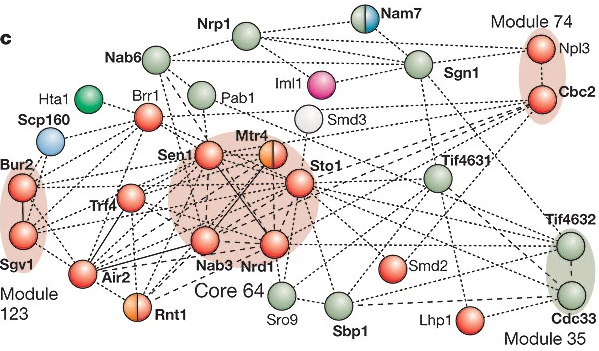
\includegraphics{core_append}
  \caption{核心附属结构示例——Core64部分为核心结构}
  \label{fig:core_append}
\end{figure}

ClusterONE算法\cite{nepusz_detecting_2012}
\subsection{监督学习方法}
\label{section:Supervision}
包括监督下的方法
\subsection{动态网络方法}
\label{section:Dynamic}


\subsection{方法总结}
\label{section:researchSummary}

\section{研究动机和思路}
\label{section:motivation}

国内外学者对复合物的识别已经提出了诸多方法,总体趋势也是趋向于融合生物数据和网络数据并达到更精确的预测,但是目前现有的方法还存在以下的不足。
\begin{itemize}
  \item 无法利用已有的先验知识。上述的研究方法主要是基于无监督方法,在复合物的研究问题上,无监督方法具有训练简单、结构明确的优点。再如今实验技术更新、生物数据量增加以及图数据挖掘算法井喷发展的情况下,无监督学习方法无法利用已有的先验知识。
  \item 复合物准确度较低。部分模型方法如RNSC算法\cite{king_protein_2004}、Clique算法\cite{spirin_protein_2003}等等具有很强的随机性,倾向于这类方法为了达到较高的复合物召回率,往往倾向于产生过量的候选复合物,导致结果的准确率的降低,大量非复合物预测成立复合物,这样的数据对以后的使用不好。
  \item 生物信息在$PIN$中融合度低。在\ref{section:appendBiology}中提到了融合生物信息的诸多方法,然而这些方法只停留在利用生物信息更改$PIN$邻边权重的层面,不同的生物信息如GO注释、基因表达信息、蛋白质保守性等数据被统一编码到了相互作用的边权重中,这个编码转换过程会丢失原有丰富的生物数据。编码过程仅仅作为$PIN$数据的预处理,生物数据无法动态地参与到复合物预测模型的框架设计中。同时,目前也没有方法将生物信息编码到蛋白质结点中,如何有效的利用结点编码增强复合物的预测质量也是一个亟待解决的问题。
\end{itemize}

针对以上的问题。
研究动机:RNSC算法\cite{king_protein_2004}削减的思想,Clique算法\cite{spirin_protein_2003}过多样本,Pereira‐Leal\cite{pereiraleal_detection_2004}融合了总体拓扑结构
\section{研究工作和成果}
\label{section:workandresult}

\section{论文组织}
\label{section:organization}